\documentclass[12pt,a4paper]{article}
\usepackage[utf8]{inputenc}
\usepackage{graphicx}
\usepackage{tikz}
\usetikzlibrary{shapes.geometric, arrows.meta, positioning, fit, calc}
\usepackage{geometry}
\geometry{margin=1in}
\usepackage{hyperref}

\title{Autonomous Sea Vehicle Ground Station\\ \Large Architecture Overview}
\author{Antigravity / Umut}
\date{\today}

\begin{document}
\maketitle

\section{Introduction}
This document provides a high-level overview of the Ground Station architecture designed to control and monitor the Autonomous Sea Vehicle. The architecture is highly modular, ensuring reliability, responsiveness, and ease of use for operators of all technical backgrounds.

\section{System Overview}
The system is divided into two primary environments: the \textbf{Autonomous Sea Vehicle} operating out in the water, and the \textbf{Ground Station} operated by the user at the base. They communicate via a secure and continuous wireless Telemetry Link.

\begin{figure}[h]
\centering
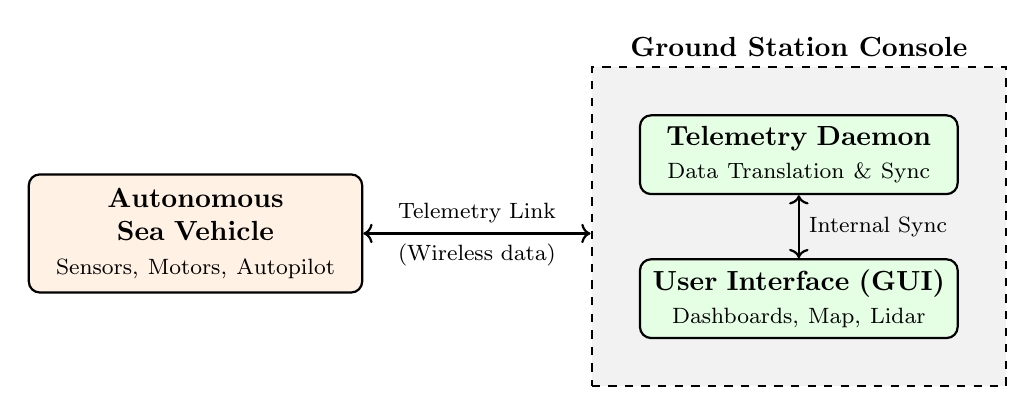
\begin{tikzpicture}[
    node distance=2cm,
    box/.style={rectangle, draw=black, thick, fill=blue!10, text width=4cm, align=center, minimum height=1.5cm, rounded corners},
    subbox/.style={rectangle, draw=black, thick, fill=green!10, text width=3.8cm, align=center, minimum height=1cm, rounded corners},
    arrow/.style={-{Stealth[scale=1.2]}, thick}
]

% Vehicle
\node[box, fill=orange!10] (vehicle) {\textbf{Autonomous Sea Vehicle} \\ \footnotesize Sensors, Motors, Autopilot};

% Ground Station Boundary
\node[subbox, right=3.5cm of vehicle, yshift=1cm] (daemon) {\textbf{Telemetry Daemon} \\ \footnotesize Data Translation \& Sync};
\node[subbox, below=0.8cm of daemon] (gui) {\textbf{User Interface (GUI)} \\ \footnotesize Dashboards, Map, Lidar};

\node[draw=black, thick, dashed, inner sep=0.6cm, fill=black!5, fit=(daemon) (gui), label=above:\textbf{Ground Station Console}] (gs) {};

% Redraw subboxes so they are on top of the black!5 fill
\node[subbox] at (daemon) {\textbf{Telemetry Daemon} \\ \footnotesize Data Translation \& Sync};
\node[subbox] at (gui) {\textbf{User Interface (GUI)} \\ \footnotesize Dashboards, Map, Lidar};

% Connections
\draw[arrow, <->] (vehicle.east) -- node[above] {\footnotesize Telemetry Link} node[below] {\footnotesize (Wireless data)} (gs.west |- vehicle.east);
\draw[arrow, <->] (daemon.south) -- node[right] {\footnotesize Internal Sync} (gui.north);

\end{tikzpicture}
\caption{High-Level System Architecture}
\end{figure}

\section{Core Components}

\subsection{1. The Graphical User Interface (GUI)}
The User Interface is the front-end dashboard where the operator visualizes the vehicle's state. It is built to be extremely fast and responsive, meaning it will never freeze while waiting for data. It provides:
\begin{itemize}
    \item \textbf{Telemetry Metrics:} Live readings of engine temperatures, battery voltage, and vehicle speed.
    \item \textbf{Environmental Data:} Display of water temperature, depth, and wave heights dynamically.
    \item \textbf{Situational Awareness:} A point-cloud map and 360-degree Lidar area to visualize the vehicle's surrounding obstacles.
\end{itemize}

\subsection{2. The Telemetry Daemon}
Running invisibly behind the scenes, the Telemetry Daemon acts as the communications manager. Because the visual user interface needs to render continuously at high frame rates, the Daemon handles the tedious heavy lifting of network connectivity:
\begin{itemize}
    \item \textbf{Listening:} Continuously listening for incoming signals from the sea vehicle over the network.
    \item \textbf{Translating:} Converting raw sensor data into a structured format that the display can easily read.
    \item \textbf{Updating:} Seamlessly passing organized updates to the GUI so the operator always sees the latest information without lag.
\end{itemize}

\subsection{3. The Autonomous Sea Vehicle}
The remote physical craft operates autonomously or via remote directives. It gathers data through its suite of sensors (GPS, Lidar, thermal probes) and repeatedly transmits this payload back to the Ground Station over the long-range telemetry link.

\section{Summary}
By separating the \textbf{Data Processing (Daemon)} from the \textbf{Visual Display (GUI)}, the Ground Station remains highly stable even when remote signal quality fluctuates or large amounts of map data are received simultaneously. This two-part structure guarantees that the operator maintains reliable, uninterrupted oversight over the Autonomous Sea Vehicle at all times.

\end{document}
